% Editable LaTeX reconstruction from the user-provided manuscript PDF.
% The original Microsoft Word/LaTeX author source was not provided.
% Scientific content, names, tables, reference order and figure imagery are
% transcribed from the supplied PDF; typesetting/pagination may differ.
% DO NOT edit reported benchmark numbers without author experimental evidence.
\documentclass[10pt,journal]{IEEEtran}
\usepackage{graphicx,amsmath,amssymb,booktabs,tabularx,array,multirow,adjustbox}
\usepackage[hidelinks]{hyperref}
\usepackage{url}
\usepackage{fontspec}
\setmainfont{Liberation Serif}
\usepackage{balance}
\usepackage{microtype}
\hyphenation{RGB-Thermal multi-modal counter-factual}
\begin{document}
\title{Cross-Modal Semantic Alignment and Counterfactual Utility-Guided Fusion for RGB-Thermal Object Detection}
\author{Baojian Ren, Tao Cao, \IEEEmembership{Member, IEEE}, Zhengyang Zhang, Jing Wu, Xinglin Zhang, and Shuchen Bai%
\thanks{Baojian Ren, Tao Cao, Zhengyang Zhang, and Jing Wu are with the School of Computer Engineering, Shangqiu University, Shangqiu 476000, China.}%
\thanks{Xinglin Zhang is also with the School of Computer Science, Universiti Utara Malaysia, Sintok, Kedah 06010, Malaysia.}%
\thanks{Tao Cao and Shuchen Bai are also with the School of Information Science and Engineering, Dalian Polytechnic University, Dalian 116034, China.}%
\thanks{Corresponding author: Tao Cao (e-mail: caotao@sqxy.edu.cn). This work was supported by the Shangqiu Municipal Science and Technology Research Program under Grant No. 2026143.}}
\maketitle


\begin{abstract}
RGB-thermal (RGB-T) object detection benefits from complementary visible and thermal cues, yet conventional dual-stream systems often apply costly cross-modal processing uniformly, regardless of its value for individual inputs. This paper proposes RD-Fuse, a lightweight, task-utility-guided framework for conditional RGB-T detection. A shallow semantic-state probe captures cross-modal disagreement and modality reliability before expensive processing. During training, counterfactual evaluations of alternative inference paths and localized interactions provide detection-loss-based supervision for predicting their task benefits. A unified budget-conditioned router jointly selects inference paths and interaction windows according to predicted gains and hardware-profiled latency, while regret-oriented optimization aligns decisions with realized task-and-computation costs. During inference, unselected deep branches and local interactions are skipped. On M3FD, RD-Fuse achieves 90.1\% mAP50 and 62.7\% mAP50:95; on LLVIP, it achieves 94.8\% and 62.2\%, respectively. On NVIDIA Jetson Orin NX, average executed computation decreases by 41.6\% to 19.8 GFLOPs, and mean latency drops by 50.3\% to 17.6 ms relative to the dual-stream baseline. These results demonstrate a favorable accuracy--efficiency trade-off for resource-constrained multimodal perception.
\end{abstract}

\begin{IEEEkeywords}
RGB-thermal perception; cross-modal semantic alignment; reliability-aware fusion; adaptive multimodal fusion; dynamic routing
\end{IEEEkeywords}

\section{Introduction}

RGB-thermal (RGB-T) perception plays an important role in robust object detection under challenging environmental conditions. Visible images provide rich texture and color information, while thermal images offer complementary cues under low illumination and nighttime conditions [1]. However, heterogeneous imaging mechanisms introduce substantial cross-modal discrepancies [2], and varying modality quality makes fixed fusion strategies vulnerable to unreliable or redundant information.

Computational efficiency further limits real-time RGB-T deployment. Existing dual-stream detectors typically execute predefined modality-specific and cross-modal operations for every input [3], regardless of their actual contribution to detection performance. Although adaptive fusion can adjust modality weights or interaction regions, its decisions often rely on reliability or semantic disagreement, which do not necessarily indicate the task-level benefit of additional computation. High disagreement may arise from either useful complementarity or modality degradation, while semantically consistent modalities may still provide valuable local information. Consequently, determining whether and where additional cross-modal computation is worthwhile remains a critical challenge, particularly on resource-constrained devices [4].

To address this challenge, we propose RD-Fuse, a lightweight framework that formulates RGB-T detection as a task-effective computation allocation problem. Instead of directly mapping semantic disagreement to predefined fusion decisions, RD-Fuse learns the detection benefits of alternative computational paths through counterfactual loss supervision. A lightweight semantic-state probe enables utility prediction before expensive deep-stage processing. Based on these predictions, a unified budget-conditioned router jointly

evaluates global inference paths and local interaction opportunities, incorporating regional gains into global route selection. Furthermore, decision-oriented regret optimization aligns computational choices with detection performance and hardware-profiled execution costs. This design enables conditional execution of selected branches and interaction windows without evaluating alternative paths during inference.

The main contributions are summarized as follows:

1) Counterfactual task-utility learning: We introduce a taskdriven utility estimation mechanism that predicts the detection gains of alternative computational paths and local interactions from early cross-modal semantic states, replacing heuristic disagreement-based decisions.

2) Unified budget-conditioned routing: We develop a joint computation allocation mechanism that incorporates regional interaction gains into global path valuation, enabling adaptive selection of inference paths and interaction windows under hardware latency constraints.

3) Decision-oriented optimization: We integrate counterfactual utility supervision with budget-aware regret minimization to improve routing decisions, while early conditional execution enables actual computation skipping during inference.



\section{Related Work}

RGB-T detection has evolved from early input- and decisionlevel fusion toward deep feature-level interaction. Recent methods employ attention, multiscale aggregation, and progressive fusion to exploit complementary visible and thermal information [5], [6], [7]. Meanwhile, cross-modal alignment techniques, including feature remapping, globallocal correspondence, and deformable alignment, have been developed to reduce representation discrepancies [8], [9], [10], [11]. Although effective for feature integration, these methods generally emphasize representation quality rather than the computational value of additional interaction.

Reliability-aware fusion has been investigated to address modality degradation and imbalance [12]. Existing approaches estimate modality quality and adaptively suppress unreliable features under adverse illumination, sensor noise, or partial modality failure [13], [14]. However, reliabilitybased weighting does not necessarily indicate whether executing an alternative computational path would improve detection performance.

Efficient RGB-T perception has also benefited from lightweight backbones, model compression, and compact fusion structures [15], [16], [17]. TDSF-NET [18] uses target-guided sparse interaction, while SFEDet [19] restricts fusion to proposal-derived RoIs. Adaptive-depth tracking [20] and reliability-conditioned routing [21] further explore inputdependent computation. In contrast, RD-Fuse uses counterfactual detection-loss gains, rather than proposal salience or modality reliability alone, to jointly select global execution paths and local interactions under hardware-profiled latency budgets.

Cost-aware routing and regret-based decision learning have been investigated in other domains [22], providing a useful foundation for task-driven computation allocation. Building on this perspective, RD-Fuse estimates counterfactual detection gains from early cross-modal representations and incorporates regional interaction utilities into global route valuation. Unlike independently optimized path and region selection, the proposed CU-Router jointly determines the computational configuration under hardware-profiled latency constraints.



\section{Proposed Method}

\subsection{Lightweight Cross-Modal Semantic State Modeling}

The proposed RD-Fuse performs conditional RGB-thermal detection by allocating computation according to its predicted task-specific benefit. As illustrated in Fig. 1, the framework consists of a lightweight semantic-state probe, counterfactual utility predictors, and a unified budget-conditioned router (CU-Router). Unlike conventional adaptive fusion methods that directly associate modality reliability or feature discrepancy with computational demand, RD-Fuse explicitly estimates the value of alternative processing operations before expensive deep-stage execution.



Given paired RGB and thermal inputs IR and IT, shallow encoders and lightweight projections produce modalityspecific representations in a shared semantic space:



\begin{equation}
Z_m=P_m\!\left(E_m^s(I_m)\right),\quad m\in\{R,T\}.
\tag{1}
\end{equation}


Here, $E_m^s$ and $P_m$ denote the shallow encoder and low-dimensional projection, respectively. To suppress modality-specific representation bias while preserving fine-grained correspondence, global and local semantic alignment are jointly optimized:

\begin{equation}
\mathcal L_{\mathrm{align}}=\lambda_g\mathcal L_g+\lambda_l\mathcal L_l.
\tag{2}
\end{equation}


Both terms employ symmetric InfoNCE objectives with a shared contrastive temperature. The global objective aligns paired scene embeddings, while the local objective aligns corresponding spatial windows and incorporates the top-$K_h$ most similar non-corresponding cross-modal regions as hard negatives. These operations establish a calibrated representation space without requiring the two modalities to become identical.

Let $g_m=\operatorname{GAP}(Z_m)$ and $\bar z_{m,i}$ denote the global and window-level representations. Global and local disagreements, $d_g$ and $d_i$, are calculated using normalized cosine distance, $[1-\cos(\cdot,\cdot)]/2$. In parallel, a lightweight shared estimator predicts relative modality reliability scores $r_m\in[0,1]$ from $g_m$ and normalized spatial activation entropy, computed from softmax-normalized mean absolute window activations. A pairwise margin-ranking loss assigns higher scores to original views than to their synthetically degraded counterparts within the same modality.



\begin{equation}
s_g=[g_R,g_T,r_R,r_T,d_g],\quad s_i=[\bar z_{R,i},\bar z_{T,i},d_i].
\tag{3}
\end{equation}


Importantly, these descriptors characterize cross-modal conditions rather than directly prescribing fusion operations. High semantic disagreement may result from complementary information, but also from corruption or misalignment. RD-Fuse therefore learns the relationship between early semantic states and the actual detection benefit of further computation.



\begin{figure*}[!t]
\centering
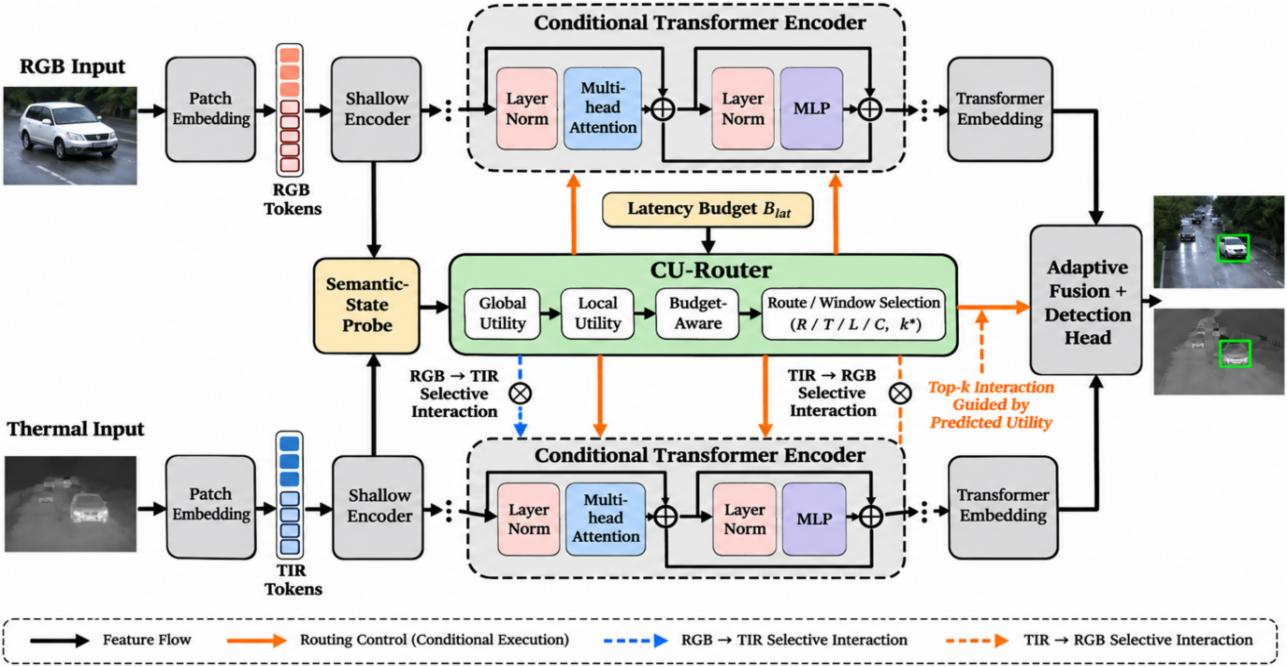
\includegraphics[width=0.94\textwidth]{figures/fig1.jpeg}
\caption{RD-Fuse architecture showing conditional deep branches and selected interaction windows.}
\label{fig:1}
\end{figure*}


\subsection{Counterfactual Task-Utility Learning}

Semantic disagreement and modality reliability describe input conditions but do not directly quantify computational benefit. RD-Fuse therefore learns to predict signed detection-loss gains through counterfactual supervision, comparing global paths against lightweight mode L and local interactions against the no-interaction mode $C_0$.

All modes share RGB/T stages 1--2, semantic probing, and a three-scale detection head. After stage 2, route-available features are projected and resampled to the head's common multi-scale interface. L uses shallow bimodal features; R/T retain one deep branch with lightweight compensation, skipping the other. C and $C_0$ execute both deep branches, but only C activates interactions in selected windows. Unselected branches and windows are skipped.



During training, alternative execution paths are evaluated on the same annotated sample. Using mode L as the reference, the detection-loss gain of configuration a is defined as



\begin{equation}
\Delta_a=\ell_L-\ell_a,\qquad\ell_a=\mathcal L_{\mathrm{det}}(f_a(x),y).
\tag{4}
\end{equation}


where $a\in\\{R,T,C_0\\}$, $f_a$ denotes the detector under the forced configuration, and $y$ represents the detection annotations. All configurations share the same detection-loss definition and image-level normalization. A positive $\Delta_a$ indicates a reduction in detection loss relative to lightweight inference, while a negative value indicates an unfavorable alternative. For region-level computation, the marginal gain of activating strong cross-modal interaction only within window i is defined as



\begin{equation}
u_i=\ell_{C_0}-\ell_{C_i}.
\tag{5}
\end{equation}


where $C_i$ differs from $C_0$ only by activating additional cross-modal interaction in window $i$; all other interaction windows remain inactive. The global and local gains are predicted from shallow semantic states:



\begin{equation}
\hat\Delta_a=G_\theta(s_g)_a,\qquad \hat u_i=G_\phi(s_g,s_i).
\tag{6}
\end{equation}


\begin{figure}[!t]
\centering
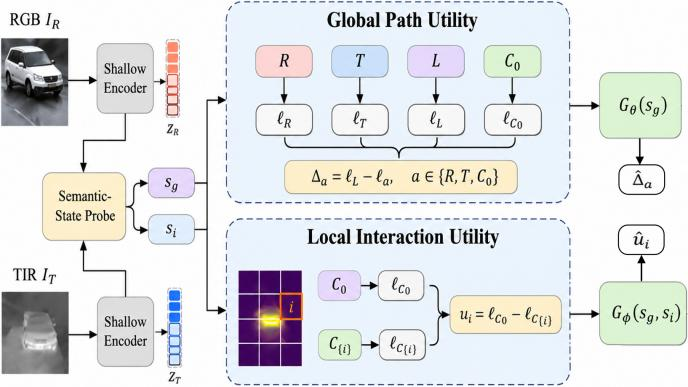
\includegraphics[width=0.95\columnwidth]{figures/fig2.jpeg}
\caption{Counterfactual task-utility learning. Global path and local interaction gains are obtained from detection-loss differences during training to supervise lightweight utility predictors.}
\label{fig:2}
\end{figure}


As illustrated in Fig. 2, counterfactual path and window evaluations provide task-level supervision for the global and

local utility predictors, respectively. The predictors are optimized by



\begin{equation}
\mathcal L_{\mathrm{util}}=\mathbb E_a[\rho(\hat\Delta_a-\Delta_a)]+\mathbb E_i[\rho(\hat u_i-u_i)].
\tag{7}
\end{equation}


where $\rho$ denotes the Huber loss, and the expectations are taken over the non-reference paths and sampled local windows. Counterfactual targets are detached during optimization and evaluated only during training. Thus, the utility predictors learn task-specific computational gains rather than relying directly on semantic disagreement.



\subsection{Unified Budget-Conditioned Computation Routing}

Independent global and local routing may overlook valuable regional interactions or activate unnecessary high-capacity computation. To address this limitation, CU-Router jointly evaluates inference paths and interaction windows under a unified utility-cost objective. For deployment device $h$, the execution latency of path a with k activated interaction windows is modeled as



\begin{equation}
C_h(a,k)=C_h^s+C_h^a+\mathbf{1}(a=C)\,C_h^w(k).
\tag{8}
\end{equation}


where $C_h^s$ covers shared shallow processing and routing, $C_h^a$ denotes the mandatory path cost including detection, and $C_h^w(k)$ represents the incremental window-processing cost, with $C_h^w(0)=0$. These costs are profiled on the target hardware, including interaction and tensor manipulation overhead. Let $\hat u_{(j)}$ denote the $j$-th largest predicted regional gain, with $\hat\Delta_L=0$ and $\hat\Delta_C=\hat\Delta_{C_0}$. The computation value is defined as



\begin{equation}
V(a,k)=\hat\Delta_a+\mathbf{1}(a=C)\sum_{j=1}^{k}\hat u_{(j)}-\lambda C_h(a,k).
\tag{9}
\end{equation}


where $\lambda$ balances detection gain and computational cost. Modes L/R/T use k = 0; $C_0$ denotes (C, 0) and is counted once, whereas C activates k > 0 windows. Given a latency budget B, CU-Router selects



\begin{equation}
(a^*,k^*)=\arg\max_{(a,k)\in\mathcal F_h(B)} V(a,k).
\tag{10}
\end{equation}


where $\mathcal F_h(B)$ contains configurations satisfying $C_h(a,k)\leq B$. The budget is assumed to admit at least one feasible path.

As illustrated in Fig. 3, regional interaction gains contribute directly to global path valuation, coupling route selection and window allocation within a single budget-constrained decision. This allows CU-Router to prioritize informative regions or bypass expensive interaction when its predicted benefit is insufficient.

The sum in (9) is a first-order surrogate for joint window utility; inter-window redundancy or synergy is accounted for at the decision level through the realized configuration losses in (11). Selected windows are processed through compact tensor gathering, while unselected operations are skipped. As the latency model relies on device profiling, the budget represents an estimated execution constraint rather than a strict per-frame guarantee.



\begin{figure}[!t]
\centering
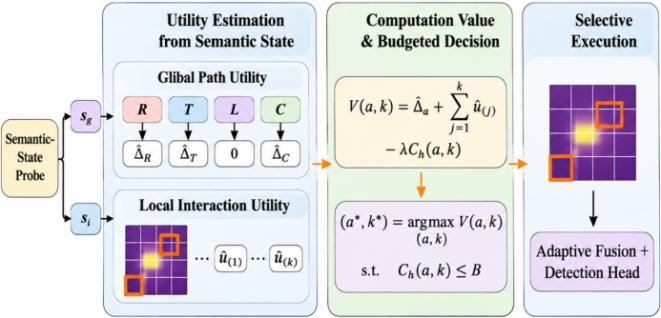
\includegraphics[width=0.95\columnwidth]{figures/fig3.jpeg}
\caption{Unified budget-conditioned routing. Global and regional utilities jointly determine the execution path and interaction windows under a latency budget.}
\label{fig:3}
\end{figure}


\subsection{Decision-Oriented Optimization and Conditional Inference}

Since additive utility estimates may misrank joint configurations, RD-Fuse minimizes budget-aware regret over sampled feasible configurations evaluated using their actual joint detection losses:



\begin{equation}
\mathcal L_{\mathrm{reg}}\triangleq\sum_{z\in\mathcal Z_{\mathrm{tr}}} p_\Psi(z\mid s_g)\left(J_z-\min_{v\in\mathcal Z_{\mathrm{tr}}}J_v\right).
\tag{11}
\end{equation}


where $z=(a,k)$ denotes a feasible path with its selected top-$k$ interaction windows, $\ell_z$ is the detection loss obtained by jointly executing the selected configuration, and $J_z=\ell_z+\lambda C_h(z)$ is the realized task-and-computation cost. Here, $\operatorname{sg}(\cdot)$ detaches regret targets, and $p_\Psi(z)=\operatorname{Softmax}_{z\in\mathcal Z_{\mathrm{tr}}}(V(z)/\tau)$, with $\Psi=(\theta,\phi)$ denoting the utility-predictor parameters. Regret gradients update both predictors through $p_\Psi$, while inference uses the hard selection in (10). The overall training objective is



\begin{equation}
\mathcal L=\mathcal L_{\mathrm{det}}+\alpha\mathcal L_{\mathrm{align}}+\beta\mathcal L_{\mathrm{rel}}+\gamma\mathcal L_{\mathrm{util}}+\delta\mathcal L_{\mathrm{reg}}.
\tag{12}
\end{equation}


where the coefficients balance detection learning, semantic alignment, reliability ranking, utility prediction, and decision-oriented optimization.

Training follows three stages. First, forced-route training initializes the conditional backbones and detection head. Second, alternative paths and sampled window interventions provide counterfactual supervision for utility prediction. Third, budget-conditioned routing is optimized with the regret objective under varying latency budgets. To control training overhead, counterfactual targets are generated with temporarily fixed detector parameters and periodically refreshed, while candidate configurations are sampled rather than exhaustively enumerated. Forced-route exploration prevents rarely selected paths from being undertrained.

During inference, counterfactual evaluations are removed. CU-Router selects the highest-value feasible path and windows from shallow semantic states, dispatching only the required TensorRT engines. Inactive deep branches are not executed; for C, attention processes only gathered top-k windows, while $C_0$ skips interaction entirely.



\section{Experimental Setup}

Experiments are configured on M3FD [23] and LLVIP [24]. M3FD contains 4,200 registered RGB-thermal pairs covering six categories; a fixed pair-disjoint split (seed 42) assigns 3,024/336/840 pairs to training, validation, and testing. LLVIP contains 15,488 pairs for pedestrian detection, with the established 12,025/3,463 training/testing partition. We reserve 1,203 training pairs for validation, leaving 10,822 for model development. All compared methods use identical data partitions and evaluation settings.

RD-Fuse adopts dual ImageNet-1K-pretrained PVTv2-B0 [25] backbones with stage channels of [32, 64, 160, 256] and a three-scale anchor-free detection head. Thermal patch-embedding weights are initialized by averaging the pretrained RGB kernels. Images are resized to 640 $\times$ 640 using letterboxing, and conditional routing is performed after the second backbone stage. The shallow features are reduced to a 40 $\times$ 40 semantic map with 64 channels, forming 64 non-overlapping windows. Global and local utility predictors employ MLP dimensions of 131--128--64--3 and 260--64--32-- 1, respectively. The selective route uses a four-head cross-modal attention block with 128 channels. Candidate interaction counts are \{0, 2, 4, 8, 12, 16\}. The shared detection head employs focal classification, GIoU regression, and centerness losses with weights of 1:2:1.

Training uses AdamW with an initial learning rate of $2\times10^{-4}$ , weight decay of 0.05, effective batch size of 16, five warm-up epochs, and cosine learning-rate decay. LLVIP is trained for 120 epochs (50/25/45 for forced-route initialization, counterfactual utility learning, and regret-aware optimization), whereas M3FD is trained for 160 epochs (70/35/55 for the same stages). Loss weights ($\alpha$, $\beta$, $\gamma$, $\delta$) are (0.10, 0.05, 0.25, 0.10), with $(\lambda_g,\lambda_l)=(0.5,0.5)$. InfoNCE temperature, hard-negative count, and reliability ranking margin are 0.07, 8, and 0.1. At each five-epoch refresh, four of 64 windows are uniformly sampled without replacement per sample; counterfactual targets are detached and computed with fixed detector parameters. The regret temperature decreases from 1.0 to 0.2; $\lambda$ is fixed at $0.005\,\mathrm{ms}^{-1}$ . Training uses synchronized geometric augmentation. With probability 0.5, either the RGB view is darkened by $b\sim U(0.6,0.9)$ or the thermal view receives Gaussian noise with $\\sigma\sim U(0.01,0.04)$, while the other modality remains unchanged.

Detection accuracy is evaluated using mAP50 and mAP50:95. Training uses RTX 4090 (24 GB; PyTorch 2.3.1, CUDA 12.1). Jetson Orin NX 16 GB (25 W, fixed clocks; TensorRT FP16, batch one) profiles costs in (8) for routing optimization. Budgets are 0.70, 0.85, and 1.00 times the profiled reference latency, excluding infeasible settings; reported results use $B=0.70T_{\mathrm{ref}}$. After 200 warm-ups, 1,000 synchronized Jetson runs measure mean and P95 end-to-end latency, including routing, interaction, and detection. Seeds: 42, 3407, 2026.



\section{Experimental Results}

\subsection{Comparison With State-of-the-Art Methods}

RD-Fuse is compared with nine representative RGB-T detectors, covering conventional dual-stream detection, multimodal integration, and recent cross-modal fusion architectures. Table I presents quantitative results on M3FD and LLVIP, while Fig. 4 illustrates qualitative feature responses under challenging conditions.



\begin{table*}[!t]\centering\caption{Quantitative Comparison of Representative RGB-T Object Detection Methods on M3FD and LLVIP (\%).}\label{tab:comparison}
\scriptsize
\begin{adjustbox}{max width=\textwidth}
\begin{tabular}{llrrrrrrrr}\toprule
& & \multicolumn{4}{c}{M3FD} & \multicolumn{4}{c}{LLVIP}\\
Method & Source & P$\uparrow$ & R$\uparrow$ & mAP50$\uparrow$ & mAP50:95$\uparrow$ & P$\uparrow$ & R$\uparrow$ & mAP50$\uparrow$ & mAP50:95$\uparrow$\\\midrule
Dual-YOLOv11s [26]&Baseline&83.6&76.1&81.4&$56.1\pm0.27$&88.9&82.7&88.5&$58.4\pm0.25$\\
Dual-RT-DETR [27]&CVPR'24&89.1&80.4&87.6&$59.0\pm0.31$&93.9&87.8&92.4&$59.1\pm0.28$\\
SuperYOLO [28]&TGRS'23&87.6&81.9&86.6&$58.3\pm0.33$&94.5&87.5&92.7&$60.7\pm0.29$\\
MMI-Det [29]&TCSVT'24&90.2&80.7&87.2&$58.4\pm0.30$&95.0&89.5&93.4&$60.3\pm0.27$\\
E2E-MFD [30]&NeurIPS'24&89.9&83.0&88.4&$59.1\pm0.28$&95.2&90.4&93.6&$62.0\pm0.25$\\
MCOR [31]&WACV'25&88.6&81.9&87.9&$57.5\pm0.32$&94.7&89.1&93.0&$61.3\pm0.29$\\
CFMW [32]&TCSVT'25&89.7&82.2&88.5&$60.1\pm0.29$&94.5&88.8&92.4&$61.4\pm0.30$\\
WaveMamba [33]&ICCV'25&90.8&83.9&89.5&$61.4\pm0.25$&95.9&91.3&94.4&$61.6\pm0.23$\\
F$^2$Net [34]&Sensors'26&91.4&84.1&89.3&$61.8\pm0.24$&96.2&91.0&94.6&$61.9\pm0.22$\\
\textbf{RD-Fuse}&Ours&91.0&84.6&\textbf{90.1}&$\mathbf{62.7\pm0.22}$&95.6&91.2&\textbf{94.8}&$\mathbf{62.2\pm0.20}$\\\bottomrule
\end{tabular}\end{adjustbox}\\[1pt]
\parbox{\textwidth}{\scriptsize Note: All methods were independently retrained on identical data splits and evaluated under a common $640\times640$ input and metric protocol; method-specific training settings were retained. Values are three-seed means; $\pm$ denotes the sample standard deviation of mAP50:95. Source indicates original publication venues; Dual-RT-DETR is a dual-stream adaptation of RT-DETR [27].}
\end{table*}

On M3FD, RD-Fuse achieves 90.1\% mAP50 and 62.7\% mAP50:95, exceeding the best competing results by 0.6 and 0.9 percentage points, respectively. It also obtains the highest recall of 84.6\%. On LLVIP, RD-Fuse achieves 94.8\% mAP50 and 62.2\% mAP50:95, exceeding the best competing results by 0.2 percentage points on both metrics (94.6\% and 62.0\%,

respectively). These results demonstrate competitive detection accuracy across both benchmarks. As illustrated in Fig. 4, RD-Fuse exhibits more spatially concentrated target-related responses across close-up, fullbody, occluded, and small-target scenarios. Compared with the selected baselines, its responses show reduced interference from surrounding regions in the illustrated examples. These qualitative observations complement the quantitative detection results in Table I.



\begin{figure*}[!t]
\centering
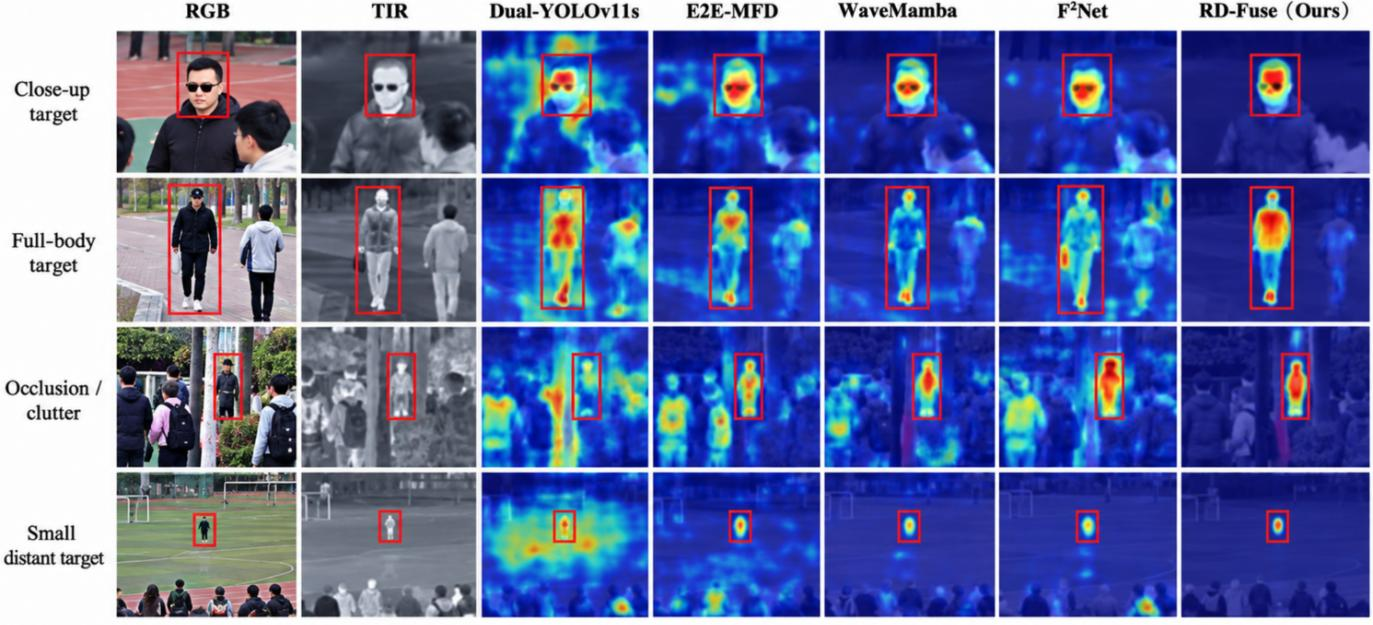
\includegraphics[width=0.94\textwidth]{figures/fig4.jpeg}
\caption{Qualitative comparison of target-related feature responses under close-up, full-body, occluded, and small distant target scenarios. Red boxes indicate selected target annotations, and warmer colors represent higher normalized responses.}
\label{fig:4}
\end{figure*}


\subsection{Computational Efficiency}

To evaluate the practical efficiency of conditional computation, representative detectors are profiled under a unified Jetson Orin NX deployment setting with TensorRT FP16 and a batch size of one. The evaluation includes routing, selective cross-modal interaction, and detection overhead. Maximum and average executed GFLOPs are reported separately to distinguish available model capacity from actual input-dependent computation.



\begin{table*}[!t]\centering\caption{Computational Complexity and Inference Efficiency of Representative RGB-T Object Detection Methods on M3FD.}\label{tab:efficiency}\small
\begin{adjustbox}{max width=\textwidth}
\begin{tabular}{lrrrrrr}\toprule
Methods & Params (M)$\downarrow$ & Max GFLOPs$\downarrow$ & Avg. GFLOPs$\downarrow$ & Mean (ms)$\downarrow$ & P95 (ms)$\downarrow$ & FPS$\uparrow$\\\midrule
MMI-Det [29]&28.3&75.1&75.1&60.8&68.1&16.4\\
E2E-MFD [30]&34.5&82.6&82.6&66.9&74.6&14.9\\
CFMW [32]&22.4&45.2&45.2&41.5&47.1&24.1\\
WaveMamba [33]&26.8&55.4&--&--&--&--\\
F$^2$Net [34]&15.4&35.6&35.6&31.5&--&31.7\\
Dual-YOLOv11s [26]&13.8&33.9&33.9&35.4&39.8&28.2\\
\textbf{RD-Fuse}&14.8&37.2&\textbf{19.8}&\textbf{17.6}&\textbf{23.9}&\textbf{56.8}\\\bottomrule
\end{tabular}\end{adjustbox}\\[1pt]
\parbox{\textwidth}{\scriptsize Note: All deployment measurements use Jetson Orin NX (TensorRT FP16, $640\times640$, batch one). RD-Fuse uses $B=0.70T_{ref}$, where $T_{ref}$ is the profiled latency of the maximum-interaction high-capacity cross-modal configuration (C, 16). Average executed GFLOPs reflect selected paths and interaction windows; latency includes routing, interaction, and detection overhead. P95 denotes the 95th-percentile latency; ``--'' indicates unavailable measurements.}
\end{table*}

As shown in Table II, RD-Fuse requires 14.8 M parameters and 37.2 maximum GFLOPs, slightly exceeding those of Dual-YOLOv11s. Nevertheless, its average executed computation decreases from 33.9 to 19.8 GFLOPs, corresponding to a 41.6\% reduction. Mean latency decreases from 35.4 to 17.6 ms, representing a 50.3\% reduction, while P95 latency reaches 23.9 ms. The resulting reciprocal-latency throughput is 56.8 FPS.

Fig. 5 further illustrates the joint relationship among detection accuracy, average executed computation, and inference latency, highlighting the favorable accuracy-- efficiency position of RD-Fuse.

These results demonstrate that RD-Fuse achieves its efficiency advantage through selective execution rather than uniform network compression. By retaining high-capacity processing for computationally demanding inputs and bypassing unnecessary operations elsewhere, the proposed framework offers a favorable balance between detection accuracy and deployment efficiency.



\begin{figure}[!t]
\centering
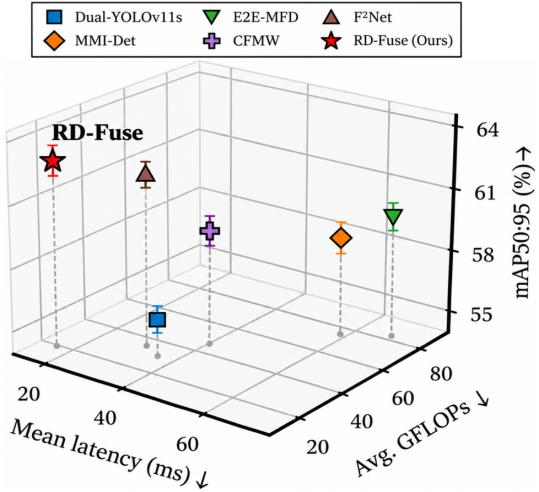
\includegraphics[width=0.95\columnwidth]{figures/fig5.jpeg}
\caption{Three-dimensional comparison of detection accuracy, average executed GFLOPs, and mean inference latency on M3FD. Error bars indicate the standard deviations of mAP50:95 over three independent runs.}
\label{fig:5}
\end{figure}


\subsection{Ablation Study}

To evaluate the proposed mechanisms, five routing variants compare heuristic estimation (H), counterfactual utility learning (U), sequential routing (S), joint budget-conditioned routing (J), and regret optimization (R). Two additional ablations disable semantic alignment or reliability modeling in the full framework. All variants share the same backbone, detection head, candidate execution paths, training schedule, and latency budget.



\begin{table}[!t]\centering\caption{Ablation Study of the Principal Components of RD-Fuse on M3FD and LLVIP.}\label{tab:ablation}\footnotesize
\begin{adjustbox}{max width=\columnwidth}\begin{tabular}{lrrrr}\toprule
Variants & M3FD mAP50:95$\uparrow$ & LLVIP mAP50:95$\uparrow$ & Avg. GFLOPs$\downarrow$ & Latency(ms)$\downarrow$\\\midrule
H+S&$60.1\pm.33$&$61.2\pm.29$&22.3&20.0\\
U+S&$60.9\pm.30$&$61.7\pm.27$&21.6&19.3\\
H+J&$60.7\pm.31$&$61.6\pm.28$&21.9&19.5\\
U+J&$62.1\pm.26$&$62.3\pm.23$&20.5&18.3\\
Full w/o Align&$61.8\pm.30$&$62.1\pm.27$&20.6&18.4\\
Full w/o Rel&$62.2\pm.25$&$62.4\pm.24$&20.1&17.9\\
U+J+R (Full)&$62.7\pm.22$&$62.2\pm.20$&19.8&17.6\\\bottomrule
\end{tabular}\end{adjustbox}\\[2pt]
\parbox{\columnwidth}{\scriptsize Note: H/U denote heuristic/counterfactual utility estimation; S/J denote sequential/joint routing; R denotes regret optimization. ``w/o Align'' sets $\alpha=0$; ``w/o Rel'' sets $\beta=0$ and fixes $r_R=r_T=0.5$. All variants share the same training protocol and latency budget. Detection results are three-seed means $\pm$ sample standard deviations; GFLOPs and latency are measured on M3FD using Jetson Orin NX (TensorRT FP16).}
\end{table}

As reported in Table III, counterfactual utility learning and joint routing independently improve M3FD mAP50:95 from 60.1\% to 60.9\% and 60.7\%, respectively. Combining both mechanisms achieves 62.1\%. Regret optimization further improves M3FD mAP50:95 from 62.1\% to 62.7\%, while maintaining comparable performance on LLVIP (62.3\% for U+J and 62.2\% for the full model). These results suggest that regret optimization primarily improves decision quality under the evaluated latency budget rather than uniformly increasing detection accuracy across datasets.



\begin{figure}[!t]
\centering
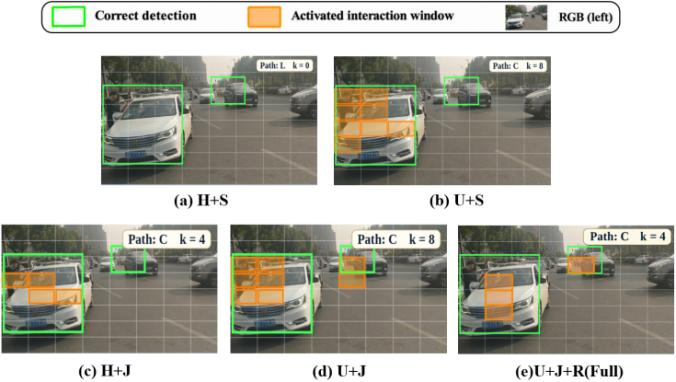
\includegraphics[width=0.95\columnwidth]{figures/fig6.jpeg}
\caption{Actual routing decisions of five ablation variants on the same M3FD sample under B = 0.70Tref: (a) H + S, (b) U + S, (c) H + J, (d) U + J, and (e) U + J + R (Full). Orange cells indicate executed interaction windows, while green boxes indicate correct detections.}
\label{fig:6}
\end{figure}


Fig. 6 compares the actual routing decisions of five variants on the same road scene, highlighting differences in computational paths and selected interaction windows. Together with the quantitative results in Table III, these observations characterize the respective roles of task-utility estimation, unified computation allocation, and decision-oriented optimization.



\subsection{Task-Utility and Routing Analysis}

To assess the effectiveness of task-driven computation allocation, we evaluate utility prediction accuracy and routing decision quality using Spearman correlation, utility mean absolute error (MAE), and decision regret. Table IV compares heuristic sequential routing (H + S), counterfactual utility learning (U + S), joint budget-conditioned routing (U + J), and the complete RD-Fuse framework.



\begin{table}[!t]\centering\caption{Task-Utility Prediction and Routing Decision Analysis on M3FD.}\label{tab:routing}\footnotesize
\begin{adjustbox}{max width=\columnwidth}\begin{tabular}{lrrr}\toprule
Routing strategy & Spearman $\rho\uparrow$ & Utility MAE$\downarrow$ & Decision regret$\downarrow$\\\midrule
Heuristic (H+S)&0.39&0.112&0.143\\
Counterfactual Utility (U+S)&0.67&0.064&0.100\\
U+Joint Routing&0.67&0.064&0.067\\
Full RD-Fuse&0.69&0.066&0.046\\\bottomrule
\end{tabular}\end{adjustbox}\\[2pt]
\parbox{\columnwidth}{\scriptsize Note: Spearman $\rho$ measures utility-ranking agreement; MAE denotes prediction error in normalized detection-loss units. Decision regret is measured against the best evaluated feasible configuration. All strategies use identical candidate sets and latency budgets, with heuristic scores calibrated on the validation set.}
\end{table}

As shown in Table IV, counterfactual utility learning increases Spearman correlation from 0.39 to 0.67 and reduces utility MAE from 0.112 to 0.064. With the utility predictor fixed, joint routing further decreases decision regret from 0.100 to 0.067. Regret-oriented optimization reduces it to 0.046, despite a slight increase in MAE, indicating that improved decision quality does not necessarily require lower utility regression error.

Fig. 7 further compares detection outputs and feature responses across distant-pedestrian, pedestrian--vehicle, and multi-pedestrian scenes. Compared with Dual-YOLOv11s, RD-Fuse exhibits more spatially concentrated target-related responses with reduced background activation in the illustrated examples. These observations complement the quantitative analysis, demonstrating competitive feature discrimination under diverse RGB-T conditions.



\begin{figure*}[!t]
\centering
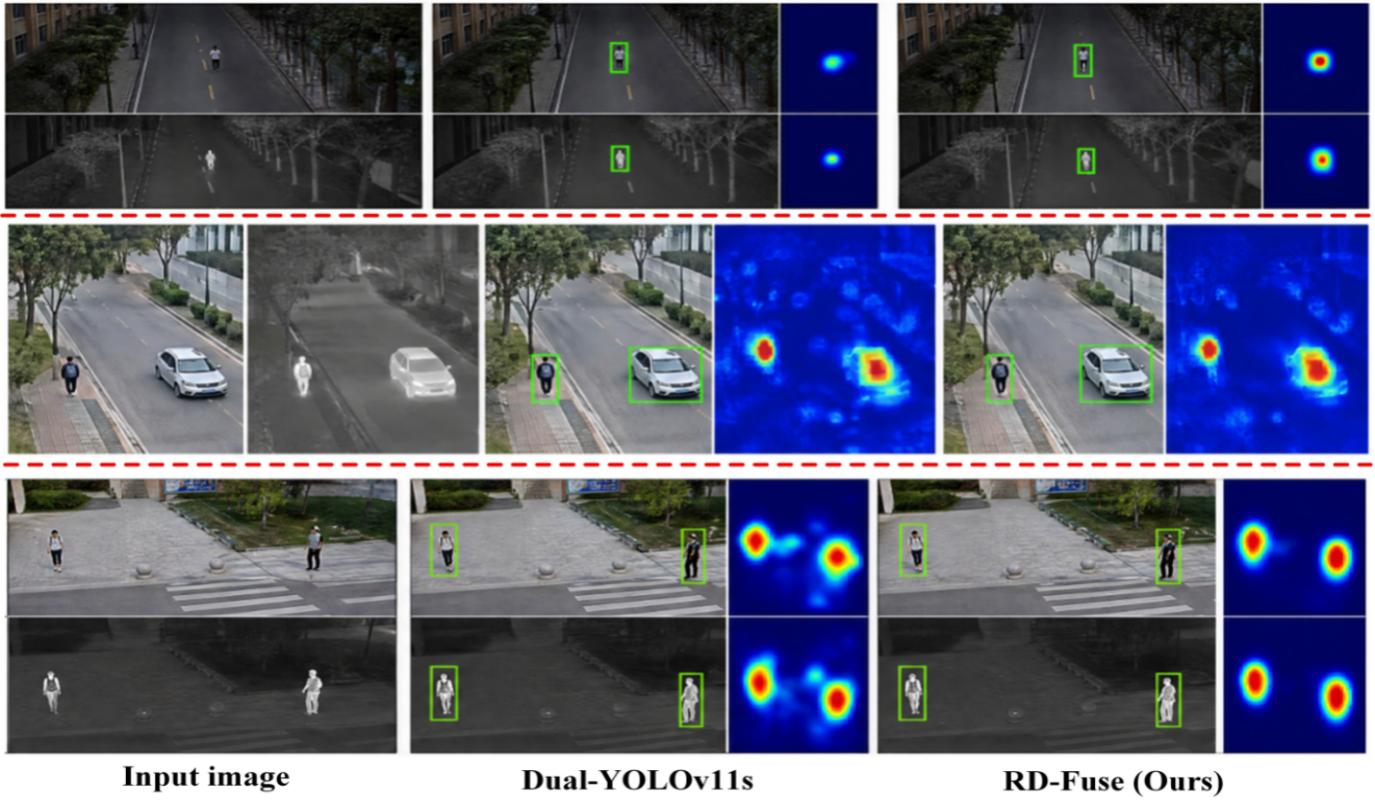
\includegraphics[width=0.94\textwidth]{figures/fig7.jpeg}
\caption{Qualitative detection and feature-response comparison between Dual-YOLOv11s and RD-Fuse across representative RGB-T scenes. Green boxes indicate detected objects, while response maps visualize target-related feature activations.}
\label{fig:7}
\end{figure*}


\subsection{Failure Case Analysis}

Despite its favorable accuracy--efficiency trade-off, RD-Fuse remains vulnerable to several challenging conditions. As illustrated in Fig. 8, severe degradation of both modalities may eliminate complementary information, resulting in missed detections and diffuse feature responses. Extremely small or occluded targets provide insufficient semantic evidence for reliable utility estimation and localization. Thermal crossover further reduces target--background separability, while substantial cross-modal misalignment can disrupt the spatial correspondence required for selective interaction.

These cases reveal the limitations of task-utility-guided computation allocation. Although CU-Router adaptively selects computational paths and interaction regions, additional processing cannot recover information absent from both modalities or fully compensate for severe geometric misregistration. Future work will investigate geometry-aware alignment, temporal information, and uncertainty-aware fallback strategies to improve robustness under such conditions.



\begin{figure}[!t]
\centering
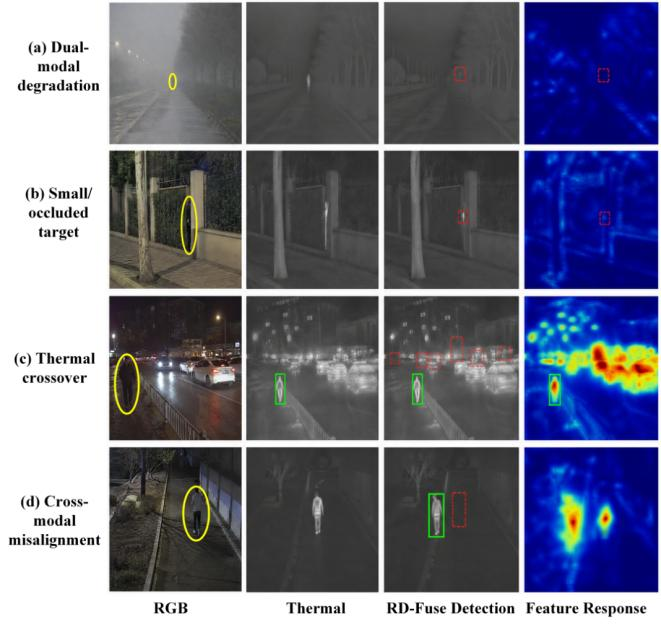
\includegraphics[width=0.95\columnwidth]{figures/fig8.jpeg}
\caption{Representative failure cases of RD-Fuse: (a) dual-modal degradation, (b) small or occluded targets, (c) thermal crossover, and (d) cross-modal misalignment. Yellow ellipses highlight target regions; green boxes indicate correct detections, while red dashed boxes mark detection failures.}
\label{fig:8}
\end{figure}


\section{Conclusion}

This paper presented RD-Fuse, a lightweight RGB-thermal detection framework that allocates computation according to predicted task utility rather than relying solely on modality reliability or semantic disagreement. Counterfactual supervision enables task-driven estimation of global path benefits and local interaction gains. A unified budgetconditioned router jointly selects inference paths and interaction windows, while regret-oriented optimization improves the quality of computational decisions.

Experiments on M3FD and LLVIP achieved mAP50:95 scores of 62.7\% and 62.2\%, respectively. On Jetson Orin NX, RD-Fuse reduced average executed computation to 19.8 GFLOPs and mean inference latency to 17.6 ms, representing reductions of 41.6\% and 50.3\% relative to the dual-stream baseline. Ablation and routing analyses further demonstrated the complementary benefits of counterfactual utility learning, unified computation allocation, and decision-oriented optimization.

Despite these improvements, severe simultaneous modality degradation, extremely small or occluded targets, and cross-modal misalignment remain challenging. Future work will investigate geometry-aware alignment and temporal information to enhance robustness while preserving the efficiency of conditional execution.



\section*{Acknowledgment}

The authors would like to thank their colleagues for their helpful discussions and constructive suggestions during this research. The authors also appreciate the technical support and computational resources provided by their institution.



\begin{thebibliography}{34}

\bibitem{ref1} Z. Zhu, X. Song, G. Zhou, M. Chen, and X. Deng, ``CAC-Net: Convolutional Additive Cross-Modal Fusion for Real-Time RGB-T Object Detection,'' IEEE Access, vol. 14, pp. 81813--81823, 2026, doi: 10.1109/ACCESS.2026.3694554.

\bibitem{ref2} J. I. Park and C. Kim, ``XGMR: Detector-Free RGB-Thermal Image Registration With Geometric Inductive Bias,'' IEEE Access, vol. 14, pp. 146741--146754, 2026, doi: 10.1109/ACCESS.2026.3735517.

\bibitem{ref3} J. E. Gallagher and E. J. Oughton, ``Surveying You Only Look Once (YOLO) Multispectral Object Detection Advancements, Applications, and Challenges,'' IEEE Access, vol. 13, pp. 7366--7395, 2025, doi: 10.1109/ACCESS.2025.3526458.

\bibitem{ref4} Z. Lin, Y. Wang, J. Zhang, and X. Chu, ``DynamicDet: A Unified Dynamic Architecture for Object Detection,'' in Proc. IEEE/CVF Conf. Comput. Vis. Pattern Recognit. (CVPR), 2023, pp. 6282--6291, doi: 10.1109/CVPR52729.2023.00608.

\bibitem{ref5} Z. Liu, C. Zhu, Y. Li, and P. Ye, ``A Novel Implicit Cross-Attention Framework for RGB-T Object Detection,'' Expert Syst. Appl., vol. 314, Art. no. 131570, 2026, doi: 10.1016/j.eswa.2026.131570.

\bibitem{ref6} X. Yang, M. Yang, and X. Xie, ``MCF-YOLO: Consistency-Guided Cross-Modal Attention for Small-Object RGB-IR Detection,'' Sensors, vol. 26, no. 12, Art. no. 3938, 2026, doi: 10.3390/s26123938.

\bibitem{ref7} H. Li, H. Xu, and D. Chen, ``MCFusion: A Lightweight RGB-T Pedestrian Detection Method With Progressive Thermal Compensation,'' Algorithms, vol. 19, no. 6, Art. no. 468, 2026, doi: 10.3390/a19060468.

\bibitem{ref8} H. Wang, Q. Yu, Z. Di, and G. Yang, ``Explicit Semantic Alignment Network for RGB-T Salient Object Detection With Hierarchical Cross-Modal Fusion,'' Image Vis. Comput., vol. 162, Art. no. 105730, 2025, doi: 10.1016/j.imavis.2025.105730.

\bibitem{ref9} M. Wu, X. Liu, X. Li, and W. Gan, ``CMGFDet: Cross-Modal Gated Fusion Network With Multi-Receptive Field Aggregation for RGB-- Infrared Aerial Object Detection,'' Remote Sens., vol. 18, no. 15, Art. no. 2439, 2026, doi: 10.3390/rs18152439.

\bibitem{ref10} X. Wen, H. Yin, K. Li, W. Nie, J. Zhao, and K. Song, ``CMAI-Det: Cross-Modal Alignment and Interaction for RGB-T Object Detection in Drone Scenes,'' IEEE Trans. Geosci. Remote Sens., vol. 63, 2025, doi: 10.1109/TGRS.2025.3645820.

\bibitem{ref11} M. Wang, F. Shi, X. Cheng, C. Jia, and S. Chen, ``Uncertainty-Aware Modality Fusion for Unaligned RGB-T Salient Object Detection,'' in Proc. IEEE/CVF Conf. Comput. Vis. Pattern Recognit. (CVPR), 2026, pp. 41489--41498.

\bibitem{ref12} L. Tian and X. Wang, ``RASM-Net: A Reliability-Aware Structural and Multiscale Modeling Network for RGB-T Object Detection in Complex Environments,'' Remote Sens., vol. 18, no. 19, Art. no. 3288, 2026, doi: 10.3390/rs18193288.

\bibitem{ref13} T. Lu, J. Lu, W. Fu, and Y. Xi, ``Illumination-Aware Multimodal Hierarchical Fusion Network for RGB-Infrared Object Detection,'' IEEE Trans. Geosci. Remote Sens., vol. 63, Art. no. 5010014, 2025, doi: 10.1109/TGRS.2025.3636590.

\bibitem{ref14} R. An, Y. Guo, Z. Wang, Z. Zhao, C. Deng, and J. Li, ``MRT-DETR: A Robust Visible--Infrared Object Detector With Adaptive Cross-Modal Feature Fusion,'' Infrared Phys. Technol., vol. 153, Art. no. 106346, 2026, doi: 10.1016/j.infrared.2025.106346.

\bibitem{ref15} J. Park, S.-W. Park, S.-H. Jung, and C.-B. Sim, ``LEAEF: Lightweight Explicit Channel-Reweighting Fusion for RGB--Thermal Perception,'' IEEE Access, vol. 14, pp. 44441--44450, 2026, doi: 10.1109/ACCESS.2026.3673767.

\bibitem{ref16} Y. Gao, X. Cheng, Y. Li, D. Xu, D. Sun, and Y. Hu, ``ISDG-Net: Efficient RGB--Infrared Object Detection for Remote Sensing Imagery,'' Remote Sens., vol. 18, no. 10, Art. no. 1570, 2026, doi: 10.3390/rs18101570.

\bibitem{ref17} B. Yu, G. Zhang, Q. Wang, and L. Wang, ``DDAF-Net: Decoupled and Differentiated Attention Fusion Network for Object Detection,'' Sensors, vol. 26, no. 6, Art. no. 1812, 2026, doi: 10.3390/s26061812.

\bibitem{ref18} J. Wang, L. Liu, J. Chen, Y. Zhang, D. Shi, and L. Deng, ``TDSF-NET: A Real-Time Target-Driven Sparse Fusion Network for RGB-Infrared Small Object Detection,'' J. Real-Time Image Process., vol. 23, no. 5, Art. no. 179, 2026, doi: 10.1007/s11554-026-01972-3.

\bibitem{ref19} C. Tian, Z. Zhou, C. Yang, G. Zhu, and Z. He, ``Efficient RGB-T Object Detection via Sparse Cross-Modality Fusion,'' in Computer Vision--ECCV 2026, LNCS, vol. 17046, 2026, pp. 541--559, doi: 10.1007/978-3-032-37281-9\_33.

\bibitem{ref20} T. Ding, H. Yang, L. Shi, J. Li, X. Hu, J. Yang, and Y. Tai, ``Adaptive Depth Lightweight RGB-T Tracking With Holistic Token Routing,'' in Proc. IEEE/CVF Conf. Comput. Vis. Pattern Recognit. (CVPR), 2026, pp. 20942--20952.

\bibitem{ref21} Y. Wu, ``Bridging Multimodal Fusion and Expert Routing via Spectral Reliability Descriptors for Robust Object Detection,'' in Proc. ACM Int. Conf. Multimedia (ACM MM), 2026. [Online]. Available: https://arxiv.org/abs/2606.01173.

\bibitem{ref22} A. Tsiourvas, W. Sun, and G. Perakis, ``Causal LLM Routing: End-to-End Regret Minimization From Observational Data,'' in Adv. Neural Inf. Process. Syst. (NeurIPS), vol. 38, 2025, doi: 10.52202/085713- 1252.

\bibitem{ref23} J. Liu, X. Fan, Z. Huang, G. Wu, R. Liu, W. Zhong, and Z. Luo, ``Target-Aware Dual Adversarial Learning and a Multi-Scenario Multi-Modality Benchmark to Fuse Infrared and Visible for Object Detection,'' in Proc. IEEE/CVF Conf. Comput. Vis. Pattern Recognit. (CVPR), 2022, pp. 5802--5811, doi: 10.1109/CVPR52688.2022.00571.

\bibitem{ref24} X. Jia, C. Zhu, M. Li, W. Tang, and W. Zhou, ``LLVIP: A Visible-Infrared Paired Dataset for Low-Light Vision,'' in Proc. IEEE/CVF Int. Conf. Comput. Vis. Workshops (ICCVW), 2021, pp. 3496--3504, doi: 10.1109/ICCVW54120.2021.00389.

\bibitem{ref25} W. Wang et al., ``PVT v2: Improved baselines with Pyramid Vision Transformer,'' Comput. Visual Media, vol. 8, no. 3, pp. 415--424, 2022, doi: 10.1007/s41095-022-0274-8.

\bibitem{ref26} G. Jocher and J. Qiu, Ultralytics YOLO11, ver. 11.0.0. Ultralytics, 2024. [Online]. Available: https://github.com/ultralytics/ultralytics.

\bibitem{ref27} Y. Zhao, W. Lv, S. Xu, J. Wei, G. Wang, Q. Dang, Y. Liu, and J. Chen, ``DETRs Beat YOLOs on Real-time Object Detection,'' in Proc. IEEE/CVF Conf. Comput. Vis. Pattern Recognit. (CVPR), 2024, pp. 16965--16974, doi: 10.1109/CVPR52733.2024.01605.

\bibitem{ref28} J. Zhang, J. Lei, W. Xie, Z. Fang, Y. Li, and Q. Du, ``SuperYOLO: Super Resolution Assisted Object Detection in Multimodal Remote Sensing Imagery,'' IEEE Trans. Geosci. Remote Sens., vol. 61, pp. 1-- 15, 2023, doi: 10.1109/TGRS.2023.3258666.

\bibitem{ref29} Y. Zeng, T. Liang, Y. Jin, and Y. Li, ``MMI-Det: Exploring Multi-Modal Integration for Visible and Infrared Object Detection,'' IEEE Trans. Circuits Syst. Video Technol., vol. 34, no. 11, pp. 11198--11213, 2024, doi: 10.1109/TCSVT.2024.3418965.

\bibitem{ref30} J. Zhang, M. Cao, W. Xie, J. Lei, D. Li, W. Huang, Y. Li, and X. Yang, ``E2E-MFD: Towards End-to-End Synchronous Multimodal Fusion Detection,'' in Adv. Neural Inf. Process. Syst. (NeurIPS), vol. 37, 2024, doi: 10.52202/079017-1658.

\bibitem{ref31} J. Jang, C. Park, H. Kim, J. Lee, and J. Paik, ``Multispectral Object Detection Enhanced by Cross-Modal Information Complementary and Cosine Similarity Channel Resampling Modules,'' in Proc. IEEE/CVF Winter Conf. Appl. Comput. Vis. (WACV), 2025, doi: 10.1109/WACV61041.2025.00914.

\bibitem{ref32} H. Li, Q. Hu, B. Zhou, Y. Yao, J. Lin, K. Yang, and P. Chen, ``CFMW: Cross-Modality Fusion Mamba for Robust Object Detection Under Adverse Weather,'' IEEE Trans. Circuits Syst. Video Technol., vol. 35, no. 12, pp. 12066--12081, 2025, doi: 10.1109/TCSVT.2025.3587918.

\bibitem{ref33} H. Zhu et al., ``WaveMamba: Wavelet-Driven Mamba Fusion for RGB-Infrared Object Detection,'' in Proc. IEEE/CVF Int. Conf. Comput. Vis. (ICCV), 2025, pp. 11219--11229, doi: 10.1109/ICCV51701.2025.01044.

\bibitem{ref34} Q. Du, M. Zhao, L. Song, M. Hu, Z. Wang, and W. Wu, ``Mitigating Spectral Imbalance and Detail Attenuation in RGB-Thermal Object Detection via Frequency-Guided Multimodal Fusion,'' Sensors, vol. 26, no. 13, Art. no. 4145, 2026, doi: 10.3390/s26134145.

\end{thebibliography}

\balance
\section*{Author Biographies}

\noindent\begin{minipage}{\columnwidth}
\includegraphics[width=0.24\columnwidth]{figures/portrait1.jpeg}\hfill\begin{minipage}[b]{0.72\columnwidth}\footnotesize\textbf{BAOJIAN REN} received the M.S. degree from Zhengzhou University of Aeronautics, China, in 2017. He is currently a Lecturer with Shangqiu University, China. His research interests include neural implicit representations, multimodal feature fusion, real-time semantic SLAM, RGB-D scene understanding, and robust visual perception. His recent work focuses on integrating geometric, appearance, and semantic information through cross-modal learning for scene understanding in complex environments. He has participated in several research projects and published papers in related areas.\end{minipage}\end{minipage}\par\medskip

\noindent\begin{minipage}{\columnwidth}
\includegraphics[width=0.24\columnwidth]{figures/portrait2.jpeg}\hfill\begin{minipage}[b]{0.72\columnwidth}\footnotesize\textbf{TAO CAO} (Member, IEEE; Member, CCF) received the M.E. degree in computer technology from Dalian Polytechnic University, China. He is currently with the School of Computer Engineering, Shangqiu University, China. His research interests include image processing, natural language processing, deep learning, and sentiment analysis. His recent work focuses on intelligent information processing and the application of artificial intelligence techniques to visual and textual data analysis.\end{minipage}\end{minipage}\par\medskip

\noindent\begin{minipage}{\columnwidth}
\includegraphics[width=0.24\columnwidth]{figures/portrait3.jpeg}\hfill\begin{minipage}[b]{0.72\columnwidth}\footnotesize\textbf{ZHENGYANG ZHANG} received the M.S. degree in agronomy from Hebei Normal University of Science and Technology, China, in 2019. He is currently an Assistant Dean and Lecturer with the School of Computer Engineering (School of Artificial Intelligence), Shangqiu University, China. His research interests include artificial intelligence, image processing, intelligent sensing, and their applications to visual perception systems. He has participated in the development of provincial and municipal research platforms and has led or participated in several scientific research projects.\end{minipage}\end{minipage}\par\medskip

\noindent\begin{minipage}{\columnwidth}\begin{minipage}[b]{\columnwidth}\footnotesize\textbf{JING WU} is currently a third-year undergraduate student majoring in computer science and technology at Shangqiu University, Shangqiu, China. His research interests include computer vision, deep learning, and multimodal object detection.\end{minipage}\end{minipage}\par\medskip

\noindent\begin{minipage}{\columnwidth}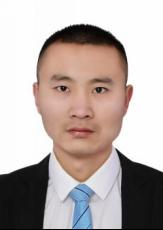
\includegraphics[width=0.24\columnwidth]{figures/portrait4.jpeg}\hfill\begin{minipage}[b]{0.72\columnwidth}\footnotesize\textbf{XINGLIN ZHANG} received the M.E. degree in computer science and technology from Universiti Utara Malaysia (UUM), Malaysia, in 2025. His research interests include the Internet of Things, smart-home systems, MIMO communications, intelligent sensing, and sensor-enabled computing. His current research focuses on the integration of communication and sensing technologies for reliable and intelligent IoT environments.\end{minipage}\end{minipage}\par\medskip

\noindent\begin{minipage}{\columnwidth}
\includegraphics[width=0.24\columnwidth]{figures/portrait5.jpeg}\hfill\begin{minipage}[b]{0.72\columnwidth}\footnotesize\textbf{SHUCHEN BAI} received the M.E. degree in computer technology from Dalian Polytechnic University, China. Her research interests include image enhancement, image processing, computer vision, and deep learning-based image restoration. Her recent work focuses on improving image quality under challenging imaging conditions, including low illumination and noise degradation, with particular interest in adaptive restoration algorithms and sensor-aware modeling for real-world imaging systems.\end{minipage}\end{minipage}\par\medskip

\end{document}
